\subsection{Truncation Breaks the Phase Invariance}\label{subsec:truncation}

A leg restricts the record to $|\tau| \leq K$. Two truncation models must be distinguished:

\begin{equation}
\begin{aligned}
\text{template truncation:}\quad y_i(t) &= \int m(\tau)\,\Phi_i(\tau - t)\,\mathbf{1}_{|\tau - t| \leq K}\,\mathrm{d}\tau, \\
\text{record truncation:}\quad y_i(t) &= \int m(\tau)\,\mathbf{1}_{|\tau| \leq K}\,\Phi_i(\tau - t)\,\mathrm{d}\tau.
\end{aligned}
\label{eq:truncation_models}
\end{equation}

$\mathbf{1}$ is the indicator function. With template truncation the record is unbounded and the templates are clipped to $K$ CPA distances about their centre. With record truncation the record is clipped to the leg and correlated with full templates. A survey leg is a record truncation, because the implementation correlates long templates ($|\tau| \leq 30$) with whatever record exists.

In both models \eqref{eq:filter_out_decomposed} still holds, with truncated correlations $c_{ij}^{K}$. Parity still gives $c_{12}^{K}(0) = c_{21}^{K}(0) = 0$, but the equal-autocorrelation identity fails. At $t = 0$ the two diagonal terms are the energies of $\Phi_1$ and $\Phi_2$ inside the pass:

\begin{equation}
\begin{gathered}
E_1(K) = \frac{2}{\pi}\Big(\arctan K + \frac{K}{1+K^2}\Big), \qquad E_2(K) = \frac{2}{\pi}\Big(\arctan K - \frac{K}{1+K^2}\Big),\\
E_1 - E_2 = \frac{4K}{\pi(1+K^2)}.
\end{gathered}
\label{eq:trunc_energy_diff}
\end{equation}

$\Phi_2$ decays as $1/\tau$ while $\Phi_1$ decays as $1/\tau^2$, so $\Phi_2$ keeps more of its energy beyond the pass: $E_2 < E_1$. $\mathbf{C}^K(t)$ is no longer a scaled rotation, and the energy acquires a term proportional to $\sin 2\beta$ that is odd in $t$. Its slope at $t = 0$ moves the maximum. To first order in $t$ (\cref{app:ep_shift}) the energy peak sits at

\begin{equation}
  \hat{\tau}_{\mathrm{EP}} \simeq \frac{4}{\pi K}\,\sin 2\beta , \qquad K \gg 1 .
  \label{eq:ep_shift}
\end{equation}

The displacement is driven by the energy imbalance $E_1 - E_2 \approx 4/(\pi K)$ between the truncated basis functions: it tilts the energy about the CPA, and the maximum moves towards the side the tilt favours, by an amount proportional to $\sin 2\beta$. Both truncation models share this law. The derivation, and its evaluation at finite $K$, are given in \cref{app:ep_shift}.

Three properties follow. The displacement vanishes for the pure phases $\beta = 0^\circ$ and $90^\circ$, i.e.\ for the horizontal and vertical components. It changes sign with $\beta$, so it cannot be averaged out over passes of unknown phase. And it decays only as $1/K$: halving it requires doubling the pass.

Equation~\eqref{eq:ep_shift} is a first-order result. The exact displacement at $\beta = 45^\circ$ exceeds it by about 30\% at $K = 5$ (0.33 against 0.25 CPA distances), 15\% at $K = 10$, 7\% at $K = 20$ and 4\% at $K = 30$ (\cref{fig:truncation}b). For short passes the higher-order terms dominate. Under record truncation, the survey case, the largest displacement over all phases and $K \geq 0.75$ is 0.65 CPA distances, at $K = 2$ and $\beta \approx 117^\circ$. Within the total-field phase range at Brest ($64$--$116^\circ$) it is 0.65, 0.28 and 0.12 CPA distances at $K = 2$, 5 and 10 (\cref{fig:truncation}c). At $d = 2$--$4$~m, 0.65 CPA distances is 1.3--2.6~m. Under template truncation the energy becomes bimodal as $\beta$ approaches $90^\circ$ at $K \approx 2$ (\cref{fig:bimodality}a), so its maximum jumps between two lobes about two CPA distances apart. Record truncation does not show this bimodality (\cref{fig:bimodality}b).

The lawnmower lines of~\cite{hleis2026obf} operated at $K \gg 10$, where the displacement is small. A snake leg of amplitude 6~m over a standoff of 2--4~m operates at $K = 1.5$--$3$, where it is largest.

\begin{figure}[t]
\centering
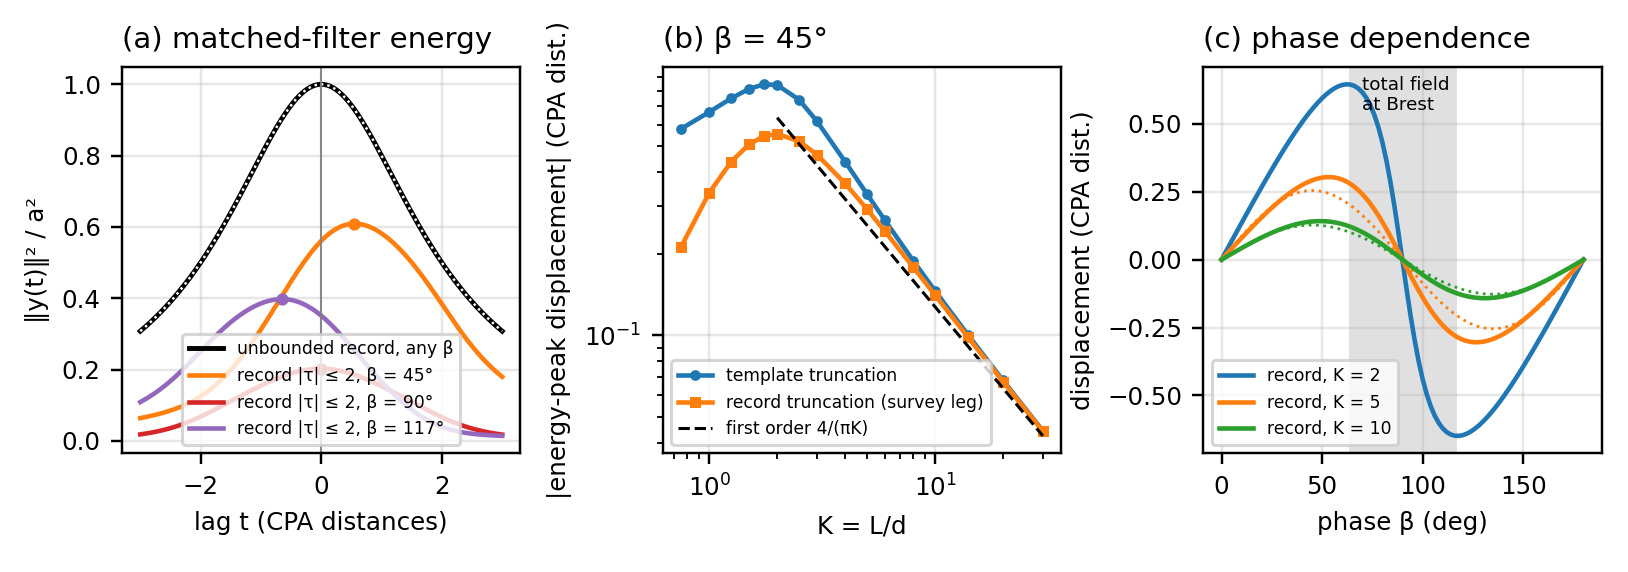
\includegraphics[width=\linewidth]{paper/sec_3_det_loc_trunc/figures/F3_truncation.png}
\caption{(a) Matched-filter energy $\|\mathbf{y}(t)\|^2/a^2$ for an unbounded record (the same curve $4/(4+t^2)$ for every $\beta$, black) and for a record truncated to $|\tau| \leq 2$ at $\beta = 45^\circ$, $90^\circ$ and $117^\circ$ (dots: maxima). (b) Energy-peak displacement at $\beta = 45^\circ$ versus $K$ for template and record truncation, with the first-order law $4/(\pi K)$. (c) Displacement versus $\beta$ under record truncation for $K = 2$, 5 and 10, with the first-order law (dotted, $K = 5$ and 10). The shaded band is the total-field phase range at Brest.}
\label{fig:truncation}
\end{figure}

\begin{figure}[t]
\centering
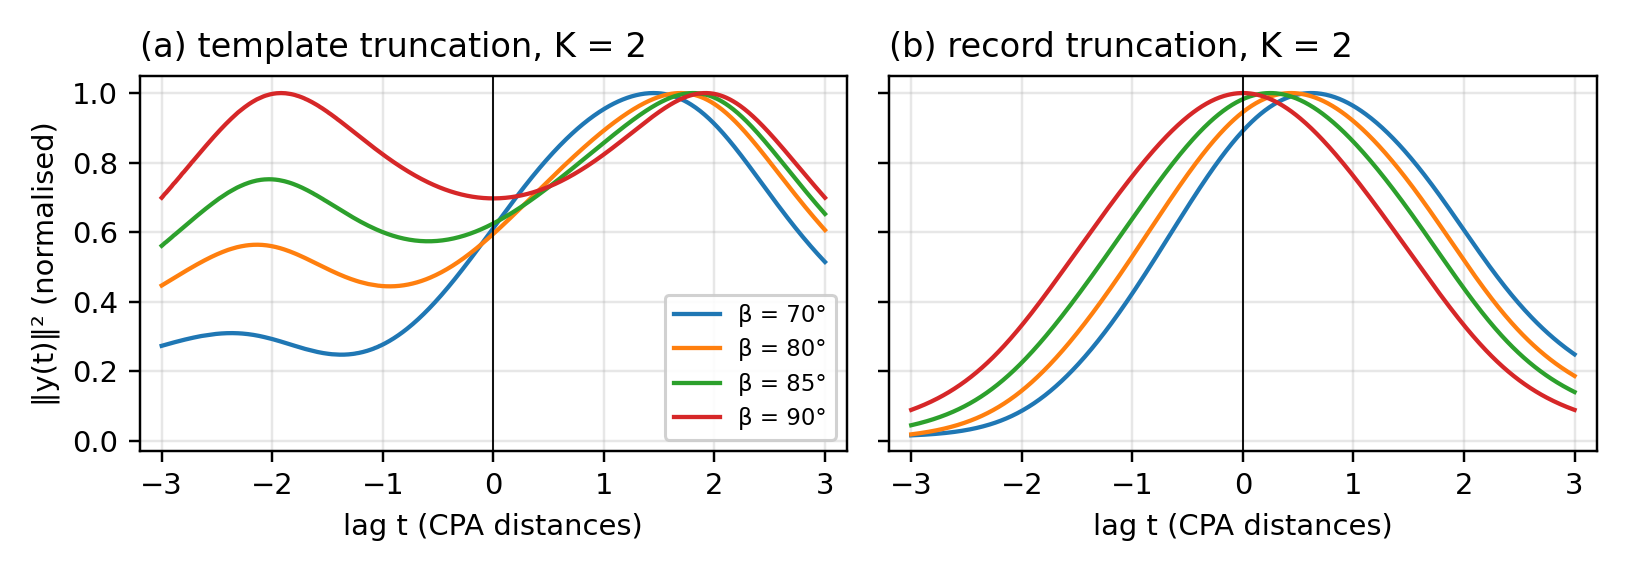
\includegraphics[width=\linewidth]{paper/sec_3_det_loc_trunc/figures/F4_bimodality.png}
\caption{Normalised energy profiles at $K = 2$ for $\beta = 70$--$90^\circ$. (a) Template truncation, which becomes bimodal as $\beta$ approaches $90^\circ$. (b) Record truncation, which does not.}
\label{fig:bimodality}
\end{figure}
